\documentclass{article}
\usepackage{amsmath}
\usepackage{amsfonts}       % blackboard math symbols
\usepackage{algorithm}      % http://ctan.org/pkg/algorithms
\usepackage{algpseudocode}  % http://ctan.org/pkg/algorithmicx
\usepackage{nicefrac}       % compact symbols for 1/2, etc.
\usepackage{graphicx}
\usepackage[font=small,skip=0pt]{subcaption}  % subcaption automatically loads caption package
\usepackage{booktabs}       % professional-quality tables
\usepackage{hyperref}       % hyperlinks
\usepackage{url}            % simple URL typesetting
\usepackage{rotating}       % sidewaystable
\usepackage[utf8]{inputenc}       % sidewaystable

\newcommand{\figref}[1]{Fig.~\ref{#1}}
\newcommand{\figrefp}[1]{(\figref{#1})}
\newcommand{\tabref}[1]{Tab.~\ref{#1}}
\newcommand{\eqnref}[1]{Eq.~(\ref{#1})}

\newcommand{\tbc}[0]{\textbf{> > > TO BE CHECKED < < <}}
\newcommand{\tbm}[0]{\textbf{> > > TO BE MODIFIED < < <}}
\newcommand{\tbe}[0]{\textbf{> > > TO BE EXPANDED < < <}}

\newcommand{\cf}[0]{\textit{cf. }}
\newcommand{\eg}[0]{\textit{e.g., }}
\newcommand{\ibid}[0]{\textit{ibid.}}
\newcommand{\ie}[0]{\textit{i.e.,}}

\newcommand{\suppmat}[0]{\hyperref[sec:supmat]{\textit{Supplementary Material}} }
\newcommand{\asuppmat}[0]{\hyperref[sec:supmat]{\textit{Sup. Mat.}} }

% Abbreviations
\newcommand{\rhs}[0]{right hand side}  % right hand side
\newcommand{\lhs}[0]{left hand side}  % left hand side
\newcommand{\snr}[0]{snr}  % signal-to-noise ratio
% Definitions
\newcommand{\realnumbers}[0]{\mathbb{R}}
\newcommand{\norm}[1]{\left\lVert#1\right\rVert}
% boldface symbols
\newcommand{\ab}[0]{\mathbf{a}}
\newcommand{\bb}[0]{\mathbf{b}}
\newcommand{\xb}[0]{\mathbf{x}}
\newcommand{\setx}[0]{\mathbf{x}_1,\ldots,\mathbf{x}_C}
\newcommand{\setxn}[0]{\mathbf{x}_1^{(n)},\ldots,\mathbf{x}_C^{(n)}}
\newcommand{\yb}[0]{\mathbf{y}}
\newcommand{\zb}[0]{\mathbf{z}}
\newcommand{\dz}[0]{d\zb}
% colored symbols
\newcommand{\xc}[0]{\color{blue}x\color{black}}
\newcommand{\xbc}[0]{\color{blue}\xb\color{black}}
\newcommand{\yc}[0]{\color{olive}y\color{black}}
\newcommand{\ybc}[0]{\color{olive}\yb\color{black}}
% bold symbols
\newcommand{\alphab}[0]{\boldsymbol{\alpha}}
\newcommand{\thetab}[0]{\boldsymbol{\theta}}
\newcommand{\thetaset}[0]{\thetab_1,\ldots,\thetab_C}
\newcommand{\phib}[0]{\boldsymbol{\phi}}
\newcommand{\phiset}[0]{\phib_1,\ldots,\phib_C}
\newcommand{\etab}[0]{\boldsymbol{\eta}}
\newcommand{\epsilonb}[0]{\boldsymbol{\epsilon}}
\newcommand{\x}[0]{\xb}
\newcommand{\xdn}[0]{\xb_{d,n}}
\newcommand{\xdnv}[0]{\xb_{d,n,v}}
\newcommand{\xdnw}[0]{\xb_{d,n,w}}
\newcommand{\z}[0]{\zb}
\newcommand{\Lin}[0]{\mathbf{L}}
\newcommand{\mub}[0]{\boldsymbol{\mu}}
\newcommand{\Sigmab}[0]{\boldsymbol{\Sigma}}
\newcommand{\sigmab}[0]{\boldsymbol{\sigma}}
% cal symbols
\newcommand{\Dcal}[0]{\mathcal{D}}
\newcommand{\Lcal}[0]{\mathcal{L}}
\newcommand{\Qcal}[0]{\mathcal{Q}}
% Gaussian
\newcommand{\Gauss}[2]{\mathcal{N}\left(#1;#2\right)}
\newcommand{\Gaussof}[1]{\mathcal{N}\left(#1\right)}
\newcommand{\Gausstd}[0]{\Gauss{\mathbf{0}}{\mathbf{I}}}
\newcommand{\GaussStdDim}[1]{\Gauss{\mathbf{0}}{\mathbf{I}_{#1}}}
% Kullback-Leibler
\newcommand{\kl}[0]{\operatorname{\mathcal{D}_{KL}}}
\newcommand{\KL}[2]{\kl\left(#1||#2\right)}
% Expected Value
\newcommand{\expect}{\operatorname{\mathbb{E}}}
\newcommand{\Var}{\operatorname{Var}}
\newcommand{\Cov}{\operatorname{Cov}}
\newcommand{\VAR}[1]{\Var\left[#1\right]}
\newcommand{\COV}[1]{\Cov\left[#1\right]}
\newcommand{\E}[1]{\expect\left[#1\right]}
\newcommand{\EE}[2]{\expect_{#1}\left[#2\right]}
% Marginal / Joint probabilities
\newcommand{\q}[1]{q\left(#1\right)}
\newcommand{\p}[1]{p\left(#1\right)}
\newcommand{\px}[0]{\p{\x}}
\newcommand{\pz}[0]{\p{\z}}
\newcommand{\pxz}[0]{\p{\x,\z}}
\newcommand{\psetx}[0]{\p{\setx}}
\newcommand{\psetxz}[0]{\p{\setx,\z}}
% Conditional probabilities
\newcommand{\pxgz}[0]{\p{\x|\z}} % x Given z
\newcommand{\psetxgz}[0]{\p{\setx|\z}}
\newcommand{\pzgsetx}[0]{\p{\z|\setx}}
\newcommand{\pzgx}[0]{\p{\z|\x}}
% Posterior
\newcommand{\pzsetx}[0]{\p{\z|\setx}}
% Variational approximation
\newcommand{\qz}[0]{\q{\z}}
\newcommand{\qzgx}[0]{\q{\z|\x}}
\newcommand{\qzgsetx}[0]{\q{\z|\setx}}
\newcommand{\qzg}[1]{\q{\z|#1}}
\newcommand{\qzx}[1]{\q{\z|\x_{#1}}}
% Lower Bound
\newcommand{\lb}[0]{\mathcal{L}}
\newcommand{\LBdnv}[0]{\lb_v^{(\xdn)}}
\newcommand{\LBdnvw}[0]{\lb_{v \leftarrow w}^{(\xdn)}}
\newcommand{\LBof}[1]{\lb\left( #1 \right)}
\newcommand{\LBn}[0]{\LBof{\xdnv}}
\newcommand{\LB}[0]{\LBof{\mathcal{D}}}
% EXPECTATION PROPAGATION
\newcommand{\qi}[0]{q_i(\thetab)}
\newcommand{\qj}[0]{q_j(\thetab)}
\newcommand{\cavity}[0]{Q_{\backslash i}(\thetab)}
% Sets
\newcommand{\set}[1]{\left\{#1\right\}}
% Optimization
\newcommand{\argmin}{\operatorname{arg\,min}}
\newcommand{\argmax}{\operatorname{arg\,max}}
\newcommand{\optim}{\operatorname{Optim}}



\begin{document}

\begin{figure}[!h]
\centering
\includegraphics[width=0.8\columnwidth]{./tex/fig/mnist_scheme.pdf}
\caption{
	Pictorial example of training imaging dataset with two views, named \textit{left} and \textit{right} views.
	In this case we have 30 independent observations:
	$10$ with left-views only; $10$ with right-views only; $10$ with complete views.
	The fraction f of observations with complete views is:
	$f = 1/3$.
}
\label{fig:mnist_scheme}
\end{figure}
%
\begin{figure}[!h]
\centering
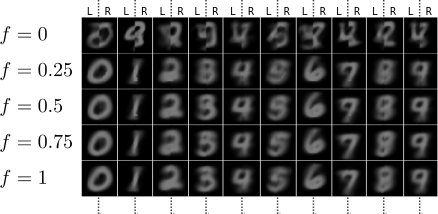
\includegraphics[width=0.8\columnwidth]{./tex/fig/mnist_half.pdf}
\caption{
	Cross reconstruction of digits with increasing degree of data availability ($f$):
	the left side of each digit is inferred from the right side and \textit{vice versa}.
}
\label{fig:mnist_half}
\end{figure}

\begin{table}
\centering
\caption{
	Mean Squared Reconstruction Error (mean (st.dev.), the lower the better) measured on clinical scores and imaging derived phenotypes predicted with our MT-MCVAE model in MTL experiments.
	Results stratified by the number of layers in the encoder-decoder architecture.
	We measure no significant differences among architectures (anova statistical test at an alpha level of 0.05).
	Best overall results in boldface.
}
\label{tab:features_mtl_nl}
\resizebox{\columnwidth}{!}{
\begin{tabular}{lllll}
\toprule
\#layers &            1 &            2 &            3 &            4 \\
\midrule
	clin    & \textbf{0.97} (0.49) &  1.05 (0.65) &  1.04 (0.60) &  1.02 (0.50) \\
	MRI     & \textbf{2.09} (0.92) &  2.14 (0.69) &  2.13 (0.68) &  2.13 (0.68) \\
	AV45    & \textbf{1.09} (0.29) &  1.16 (0.25) &  1.15 (0.26) &  1.15 (0.25) \\
\bottomrule
\end{tabular}
}
\end{table}

\begin{table}
\centering
\caption{
	Diagnosis classification accuracy (mean \% (st.dev.), the higher the better) of subjects with Alzheimer's Disease (AD), Mild Cognitive Impairment (MCI) and Normal Cognition (NC) with our model (MTL) from clinical and imaging derived phenotypes.
	Results stratified by the number of layers in the encoder-decoder architecture.
}
\label{tab:classifier_mtl_nl}
\resizebox{\columnwidth}{!}{
\begin{tabular}{cccccc}
\toprule
	                      &  \#layers   &            1   &            2   &            3   &            4  \\
\midrule
	classification task   &  condition  &                &                &                &               \\
\cmidrule(lr){1-2}
	AD vs NC              &  MTL (avg)  &  \textbf{85.79} (3.26)  &  79.04 (5.56)  &  79.78 (5.92)  &  82.47 (4.11) \\
	AD vs MCI             &  MTL (avg)  &  \textbf{59.89} (2.94)  &  56.93 (5.02)  &  56.55 (5.33)  &  57.49 (6.03) \\
\bottomrule
\end{tabular}
}
\end{table}
\end{document}
